\subsubsection{Discretización de las probabilidades de disparo}

Para obtener eventos de spikes discretos a partir de las probabilidades inferidas, se aplicó un procedimiento de ajuste por fuerza bruta. El kernel gaussiano utilizado para suavizar la verdad fundamental se utilizó como prior para la tasa de spike inferida que corresponde a un solo potencial de acción. El ajuste, por lo tanto, consistió en ajustar de forma óptima un conjunto de kernels gaussianos del ancho y la altura esperados a la tasa de spike inferida. Se realiza una primera conjetura que luego se optimiza mediante modificaciones aleatorias. La primera conjetura se generó utilizando muestreo de Monte Carlo con importancia, de modo que el número total de spikes discretos coincidía con la integral de las probabilidades inferidas. A continuación, los eventos se clasificaron en función de cómo contribuían al ajuste comparando la calidad del ajuste cuando se omitían eventos individuales. Los eventos de menor rango se descartaron y se reemplazaron por nuevos eventos, nuevamente utilizando muestreo de importancia basado en la distribución de probabilidad residual. Finalmente, cada spike se desplazó aleatoriamente durante todo el período, y se utilizó el mejor ajuste. Este enfoque es relativamente lento pero da como resultado un ajuste confiable. Para acelerar el procedimiento, las probabilidades de spike se dividieron en secuencias continuas de soporte no cero (estrategia de dividir y conquistar). 



\begin{enumerate}
	
	\item  A cada serie temporal $\Delta F/F_0$ de la actividad neuronal del experimento   se calcula sus derivadas temporales suavizadas con el método de Total-Variation Regularization  el cual es abordado en el \cref{C:ap1}. Para encontrar el parámetro de regularización  $\alpha$ optimo adoptamos un enfoque basado en principios y se utiliza un marco de optimización multiobjetivo para elegir los parámetros que minimizan una función de pérdida para equilibrar la fidelidad y la suavidad de la estimación de la derivada.  La función de pérdida para encontrar los parámetros óptimos esta dada por la \cref{eq:ap:1}, donde $\mathbf{y}$  son las series temporales, $\mathbf{\hat{\dot{x}}}$ es la estimación de la derivada,  $\text{trapz}(\cdot)$ es la integral numérica trapezoidal en tiempo discreto,  $\mu$	es la constante de integración desconocida,  $\gamma$ es un hiperparámetro, y  $TV$  es la variación total dada por la \cref{eq:ap:2}.  Para encontrar el parámetro $\gamma$ que minimiza a la \cref{eq:ap:1}   Van Breugel et al \cite{van_breugel_numerical_2020} propusieron que la mejor elección de $\gamma$ depende del contenido frecuencial de los datos. En resumen, la elección óptima de $\gamma$ , suponiendo que se valora tanto un RMSE bajo como una baja correlación de errores, puede hallarse según la siguiente relación: 
	
	
	\begin{equation}\label{eq:84}
		\log (\gamma) = -1.6\log (f) -0.71\log (dt) -5.1.
	\end{equation}
	
	A partir de los espectros de potencia que serán calculados mediante la función  de Scipy \textbf{scipy.signal.periodogram}, seleccionamos una frecuencia $f$ correspondiente a aquella en la que la potencia empieza a disminuir y el ruido del espectro aumenta. Aunque un tanto arbitrario, este enfoque (junto con la \cref{eq:84}) nos permite utilizar una herramienta estándar de procesamiento de señales para determinar rápidamente una elección de $\gamma$. Para facilitar la aplicación a nuestros datos del anterior marco de optimización utilizamos la biblioteca de Python de código abierto, \textbf{pynumdiff} \footnote{La documentación se puede encontrar en  el siguiente enlace \url{https://github.com/florisvb/PyNumDiff}}.  El  objetivo de este paquete es desarrollar un enfoque general para elegir metódicamente parámetros que equilibren la necesidad de minimizar tanto el error como el sesgo. 
	
	\item Para todas las detecciones de los picos, tanto en las  derivadas como en los datos de las series temporales, adoptamos el siguiente enfoque
	\begin{itemize}
		\item Mediante la función de  de Scipy   \textbf{scipy.signal.find\_peaks} detectamos máximos y mínimos locales en cada serie temporal: los picos máximos se encontraron como valores máximos que iban precedidos y seguidos de valores mínimos separados del máximo por una diferencia de amplitud de al menos delta, un parámetro clave.  La detección de picos implica un compromiso entre falsos positivos y falsos negativos; el parámetro delta determina lo liberal (más falsos positivos) o conservadora (más falsos negativos) que es la detección de picos. Se ha desarrollado un método sencillo para determinar automáticamente un valor de delta casi óptimo (es decir, que minimice tanto los falsos positivos como los falsos negativos). Para cada serie temporal   se realiza lo siguiente,  
		
		\begin{enumerate}[label=(\roman*)]
			\item realizamos la detección de picos con un amplio rango de deltas  que va desde demasiado liberal (muchos falsos positivos, debido a la detección de ruido) a demasiado conservador (muchos falsos negativos, algunos picos de gran amplitud no serán detectados). 
			\item graficamos el número de picos detectados en función de delta. La forma de esta curva varía en función de la serie temporal, pero a menudo se asemeja a una función lineal definida a trozos  de dos partes. En valores bajos de delta, la pendiente es alta: el número de picos detectados  está dominado por falsos positivos debido al ruido y, en este caso, pequeños aumentos de delta provocan grandes disminuciones del número de picos detectados. En valores altos de delta, la pendiente es baja: los picos detectados  son sólo reales (es decir, de gran amplitud) y, en este caso, pequeños aumentos de delta suelen dar lugar a poco o ningún cambio en el número de picos detectados. Por lo tanto, la pendiente de la curva en valores delta altos está mucho más cerca de 0 que en valores delta bajos.  En el caso ideal, el punto de cambio entre estas dos líneas es claro, dando un valor delta óptimo en el que se minimiza el número tanto de falsos positivos como de falsos negativos. 
			\item Suavizamos la curva de picos utilizando un filtro de Savitzky-Golay utilizando la función de Scipy \textbf{scipy.signal.savgol\_filter} . La principal ventaja de esta aproximación es que tiende a preservar características de la distribución inicial tales como los máximos y mínimos relativos, así como el ancho de los picos, que normalmente desaparecen con otras técnicas de promediado (como la media desplazada).
			\item Para detectar el punto de cambio utilizamos uno de los algoritmos disponibles para la detección  de múltiples puntos de cambio en series temporales multivariadas revisados por  Truong et al \cite{truong_selective_2020}.   Truong et al adoptaron una estrategia metodológica general. Los algoritmos de detección considerados se caracterizan por tres elementos: una función de coste, un método de búsqueda y una restricción sobre el número de cambios. Cada uno de estos elementos se describe, revisa y discute por separado en el articulo original  \cite{truong_selective_2020}. Las implementaciones de los principales algoritmos descritos en este artículo se proporcionan dentro de un paquete de Python llamado \textbf{ruptures}\footnote{La documentación de la librería se encuentra en: \url{https://centre-borelli.github.io/ruptures-docs/}}  el cual utilizamos en nuestros datos. Utilizamos el algoritmo que produce  el índice de la curva en la que tanto la media como la pendiente cambian más abruptamente.
		\end{enumerate}
		
		\item Para la detección de picos en derivadas, se realizaron dos pasos adicionales:
		\begin{enumerate}[label=(\roman*)]
			\item se excluyeron los picos con amplitudes inferiores a 0, ya que se trata de cambios en la pendiente de una caída y no de subidas; 
			\item el segundo de dos máximos posteriores sólo se incluyó si el mínimo intermedio caía por debajo de 0. Si el mínimo intermedio no caía por debajo de 0, los dos picos correspondían a cambios en la pendiente y no a picos de calcio individuales, por lo que se excluyó el segundo pico.
		\end{enumerate}
		
	\end{itemize}
\end{enumerate}


% derivadas 

\subsection{Calculo de las derivadas}


Aplicar diferencias finitas convencionales en los datos experimentales amplificará en gran medida cualquier ruido presente  (ver \Cref{f:derivada_diferencias_experimentos} ). La eliminación del ruido antes o después de la diferenciación no suele dar resultados satisfactorios. Un método que da buenos resultados es regularizar el propio proceso de diferenciación. Esto garantiza que la derivada calculada tendrá cierto grado de regularidad, hasta un punto que a menudo se puede controlar ajustando los parámetros. El marco que adoptaremos se encuentra en el \cref{C:ap1}. Sin embargo, el nivel y el tipo de regularización suelen imponerse de forma ad hoc, por lo que actualmente no existe un \textquote{mejor método} consensuado para obtener las derivadas \textquote{mejor ajustadas}. Para solventar este problema utilizamos un marco de optimización multiobjetivo para elegir los parámetros que equilibra dos métricas independientes.  Este enfoque minimiza una función de pérdida consistente en una suma ponderada de dos métricas calculadas a partir de la estimación de la derivada: la fidelidad de la integral de la derivada y su suavidad (\Cref{eq:ap:1}). Van breugel et al \cite{van_breugel_numerical_2020} sugieren estas métricas como aproximaciones para minimizar el error y el sesgo de la derivada estimada, y mostraron  que el barrido a través de los valores de un único hiperparámetro $\gamma$ produce estimaciones de la derivada que generalmente trazan el frente de Pareto de soluciones que minimizan el error y el sesgo. Es importante destacar que este marco de optimización no asume ningún conocimiento de la verdadera derivada subyacente y reduce la tarea de seleccionar muchos parámetros de cualquier algoritmo de diferenciación a la resolución de una función de pérdida con un único hiperparámetro. 



\begin{figure}[h!]
	\centering{}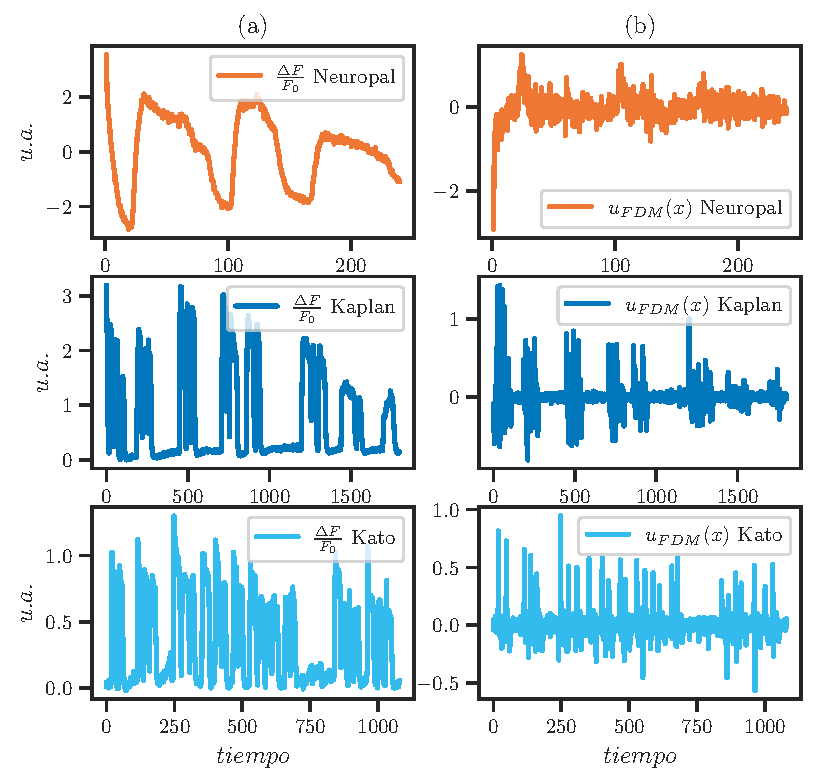
\includegraphics[width=\imsize]{derivada_diferencias_experimentos.pdf}
	\caption[Serie temporal $\Delta F/F_0$ de la neurona AVAL. (b) Resultados de la derivada en diferencias finitas  para la neurona AVAL  en cada uno de los 3 experimentos considerados.]{Serie temporal $\Delta F/F_0$ de la neurona AVAL. (b) Resultados de la derivada en diferencias finitas  para la neurona AVAL  en cada uno de los 3 experimentos considerados. Este método en todos los caso produce estimaciones de derivadas que son demasiado ruidosas para ser útiles. Por  tanto, se requieren métodos más sofisticados para el suavizado de datos y/o la diferenciación de mediciones de series temporales ruidosas.}\label{f:derivada_diferencias_experimentos}  
\end{figure}


En este apartado,  se utilizara  una heurística sencilla que es explicada en \cite{van_breugel_numerical_2020} para determinar un valor de $\gamma$ que se deriva del espectro de potencia y la resolución temporal de los datos. Todo este procedimiento se implementara  con el conjunto de herramientas Python de código abierto, pynumdiff.  Descubrimos que la mejor elección de $\gamma$ depende del contenido frecuencial de los datos.   En primer lugar, examinamos los espectros de potencia de los datos para elegir una frecuencia de corte que corresponda al inicio de la caída de potencia.  La \Cref{f:espectro_potencias_experimentos} muestra los espectros de potencia de los datos, indicando la frecuencia de corte (rojo) utilizada para seleccionar $\gamma$.  En cada conjunto de datos  la magnitud del ruido no cambia, esto se ve evidenciado  en que en un mismo experimento tanto los  espectro de potencias y la frecuencia de corte de las series neuronales son similares.  Esta frecuencia de corte, junto con la resolución temporal de los datos, se utilizan como entradas de la  heurística descrita por la \Cref{eq:84} para determinar un valor óptimo de $\gamma$.  

\begin{figure}[h!]
	\centering{}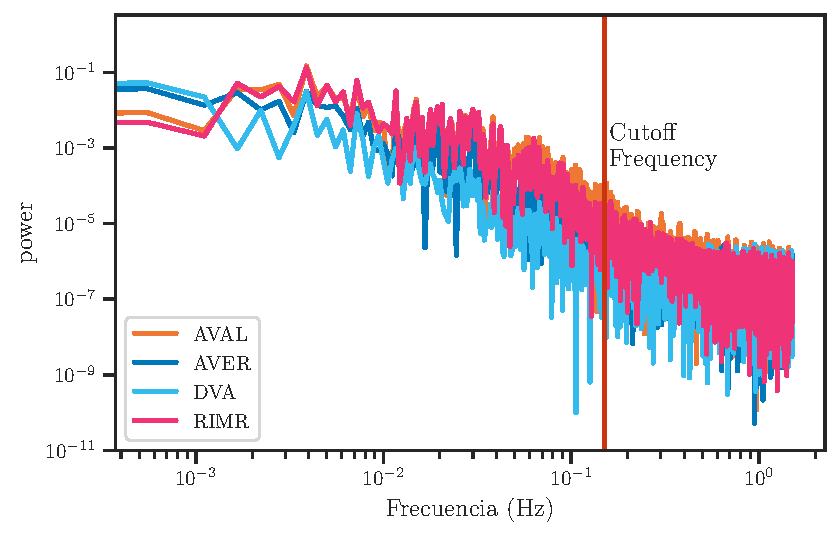
\includegraphics[width=\imsize]{espectro_potencias_experimentos.pdf}
	\caption[La frecuencia de los datos se evalúa inspeccionando los espectros de potencia; la línea roja indica la frecuencia utilizada para determinar $\gamma$]{La frecuencia de los datos se evalúa inspeccionando los espectros de potencia algunas neuronas de las series neuronales correspondientes a  los experimentos (a) Neuropal (b) Kaplan (c) Kato ; la línea roja indica la frecuencia utilizada para determinar $\gamma$. }\label{f:espectro_potencias_experimentos}  
\end{figure}


Con $\gamma$ elegido, minimizamos nuestra función de pérdida de la \Cref{eq:ap:1} para encontrar los parámetros óptimos para la diferenciación numérica.   Para mostrar el correcto  funcionamiento de este marco de optimización  en nuestros datos,  se detalla  el proceso de calcular la derivada   de la serie temporal de la neurona AVAL de uno de los cinco gusanos de los experimentos de Kaplan \cite{kaplan_nested_2020}.  La  \Cref{f:derivada_kaplan}(a) muestra la actividad de esta neurona. A partir del espectro de potencia, elegimos una frecuencia de corte de   \qty{0.15}{\hertz} (\Cref{f:espectro_potencias_experimentos}(c)). Esta selección, junto con la resolución temporal de $0.33$ segundos, produjo un valor óptimo de $\gamma=0.2787$ utilizando la  heurística descrita anteriormente.  Finalmente calculamos las estimaciones de la serie neuronal suavizada (\Cref{f:derivada_kaplan}(a))   y su derivada utilizando   tres distintos métodos de diferenciación (filtro de Savitzky-Golay , Kalman smoother y  TVR) (\Cref{f:derivada_kaplan}(b)). El resultado más significativo de este análisis es que los tres métodos, a pesar de ser muy diferentes en su matemática subyacente, se comportan de forma similar. Las únicas diferencias es en la suavidad de los picos de menor amplitud,  en  donde el método de Kalman smoother presenta la mayor suavidad. Esta similaridad entre los resultados de métodos tan distintos nos sugiere que la heurística de elección de parámetros es adecuada. En consecuencia podemos utilizar el marco de optimización para encontrar el parámetro optimo de regularización que nos permite calcular   las derivadas  regularizadas en nuestros datos. 


\begin{figure}[h!]
	\centering{}\includegraphics[width=\imsize]{derivadas_kaplan.pdf}
	\caption[Diferenciación numérica de la serie de tiempo de la neurona Aval de uno de los 5 gusanos de los experimentos de Kaplan.]{Diferenciación numérica de la serie de tiempo de la neurona Aval de uno de los 5 gusanos de los experimentos de Kaplan. (a) Serie temporal  y su valor  suavizado. (b) Derivada de los datos, utilizando un filtro Savitzky-Golay (rosado), constant acceleration Kalman forward-backward smoother  (verde), y total variation regularized jerk (naranja). Obsérvese la similitud entre los cuatro métodos.}\label{f:derivada_kaplan}  
\end{figure}


\subsection{Binarización de la actividad neuronal}

Habiendo elegido un  parámetro $\gamma$ optimo  siguiendo la heuristica descrita anteriormente,   en esta parte se muestran los resultados de umbralizar la dinámica neuronal de los experimentos con el método descrito en el \cref{sec:umbralizacion}. Se tomara como ejemplo  la serie temporal  como  su derivada de la neurona AVAL  del  experimento de Kaplan descrito anteriormente.  Este método depende de dos parámetros. En primer lugar, todos los métodos de detección de picos dependen en gran medida del grado de suavizado de los datos, que se logra en nuestro caso ajustando el hiperparámetro $\gamma$. En segundo lugar, la gama de deltas probados determina si este método tendrá éxito o no. Si el intervalo de deltas está dominado por deltas demasiado bajos o demasiado altos, no encontrará un punto de cambio adecuado, o el punto de cambio será demasiado liberal o demasiado conservador para todas las trazas. Se ha  comprobado que un único rango de deltas funciona bien para todos los datos en un determinado régimen de ruido (por ejemplo, frecuencia de muestreo, grado de suavizado) y amplitud (por ejemplo, derivada o no derivada).

En nuestros datos probamos

216.29
0.32

\cite{rupprecht_database_2021}














